% Time form: Past tense

\newpage
\chapter{Service and Tooling}\label{ch:services-and-tooling}
During the risk assessment~\ref{subsec:risk_assessment} we identified that the \glsxtrshort{AI} tokens required to use cloud based \glsxtrshort{LLM}s might be very expensive, and it's really hard to estimate the costs.
One of the possibilities to avoid this risk was the usage of self-hosted \glsxtrshort{LLM}s, and luckily we already had existing hardware at home which is suitable for running smaller \glsxtrshort{LLM}s.
Besides eliminating the costs for \glsxtrshort{AI} tokens, at least during the development phase, it also allows the quick evaluation of different \glsxtrshort{AI} Models.
Depending on the quality and performance of the smaller models running in the self-hosted setup we can consider not using a cloud based \glsxtrshort{LLM} at all.

\todo{Refactor the section: Move all information in their respective sections, etc.}

\section{Hardware Setup}\label{sec:hw_setup}

\begin{table}[h]
    \centering
    \begin{tabular}{ll}
        \hline
        \textbf{Component} & \textbf{Specification}                                  \\
        \hline
        CPU                & AMD Ryzen 7\ 1700                                       \\
        GPU                & NVIDIA GeForce RTX 3090 (24 GB \glsxtrshort{VRAM})      \\
        System Memory      & 64 GB RAM                                               \\
        \hline
    \end{tabular}
    \caption{Hardware configuration of the self-hosted \glsxtrshort{LLM} inference server.}
    \label{tab:llm_hardware_setup}
\end{table}

The 24 GB \glsxtrshort{VRAM} of the RTX 3090 allows us to run models with up to ~30 billion parameters,
depending on the specific model~\cite{simplr2025vramllm}.

\section{System Setup}\label{sec:system_setup}

The system setup described in~\ref{lst:self-hosted-base-setup-instructions} will configure and expose the Ollama \gls{API} and OpenWeb UI via NGINX,
which provided a chat \gls{GUI} to interact with Ollama.
In contrast to Ollama, which runs directly on the host, the other services are run in containers managed by rootles podman and defined the docker-compose.yml~\ref{lst:nginx-and-lets-encrypt-compose-yml}.
The \gls{Nginx} default.conf~\ref{lst:open-webui-nginx-conf} configures the web server to terminate the SSL connection and
act as reverse proxy for the \enquote{Open WebUI} and the Ollama \gls{API} under the directory \mintinline{bash}{/llm/}.

\paragraph{Services:}
\begin{itemize}
    \item Ollama: \glsxtrshort{LLM} manager, exposing an \gls{API} for prompts and other interactions (host).
    \item Swag: \gls{Nginx} web server with Certbot for automated SSL certificate generation (containerized).
    \item Open WebUI: Web based chat interface for \glsxtrshort{LLM} managers (containerized).
\end{itemize}

\newpage

\section{System Hardening}\label{sec:system_hardening}

It is recommended to put a proper firewall before the services we want to expose to the internet,
but for our purposes we can just disable the port forwarding when we don't use the \glsxtrshort{AI}.
It still makes sense to perform a minimal system hardening as shown in the following listing~\ref{lst:ufw-configuration},
before exposing the services to the internet.

\begin{listing}[H]
    \begin{minted}{bash}
# Install UFW
sudo pacman -Syu ufw
sudo ufw status

# Allow SSH for remote access
sudo ufw allow ssh

# Allow HTTP for certbot HTTP challange
sudo ufw allow http

# Allow HTTPS for Open WebUI
sudo ufw allow https

# Allow default Ollama port
sudo ufw allow 11434/tcp

# Make sure to run this command after adding the "allow" rules!
sudo ufw enable

sudo ufw status
    \end{minted}
    \caption{UFW configuration}
    \label{lst:ufw-configuration}
\end{listing}

\section{Expose Open WebUI and Ollama}\label{sec:expose-openwebui-and-ollama}

For exposing the services from the home network via HTTPS to the internet, we need a domain name which points to the home router.
To achieve this we can use DynDNS, which is provided for free by~\gls{Infomaniak} where the domain \enquote{hiube.ch} was registered, and is supported by the \gls{FRITZ!Box} used in the home network.
The screenshots~\ref{fig:infomaniak_dyndns_setup} and~\ref{fig:fritzbox_dyndns_setup} are showing the respective configurations.

\begin{figure}[H]
    \centering
    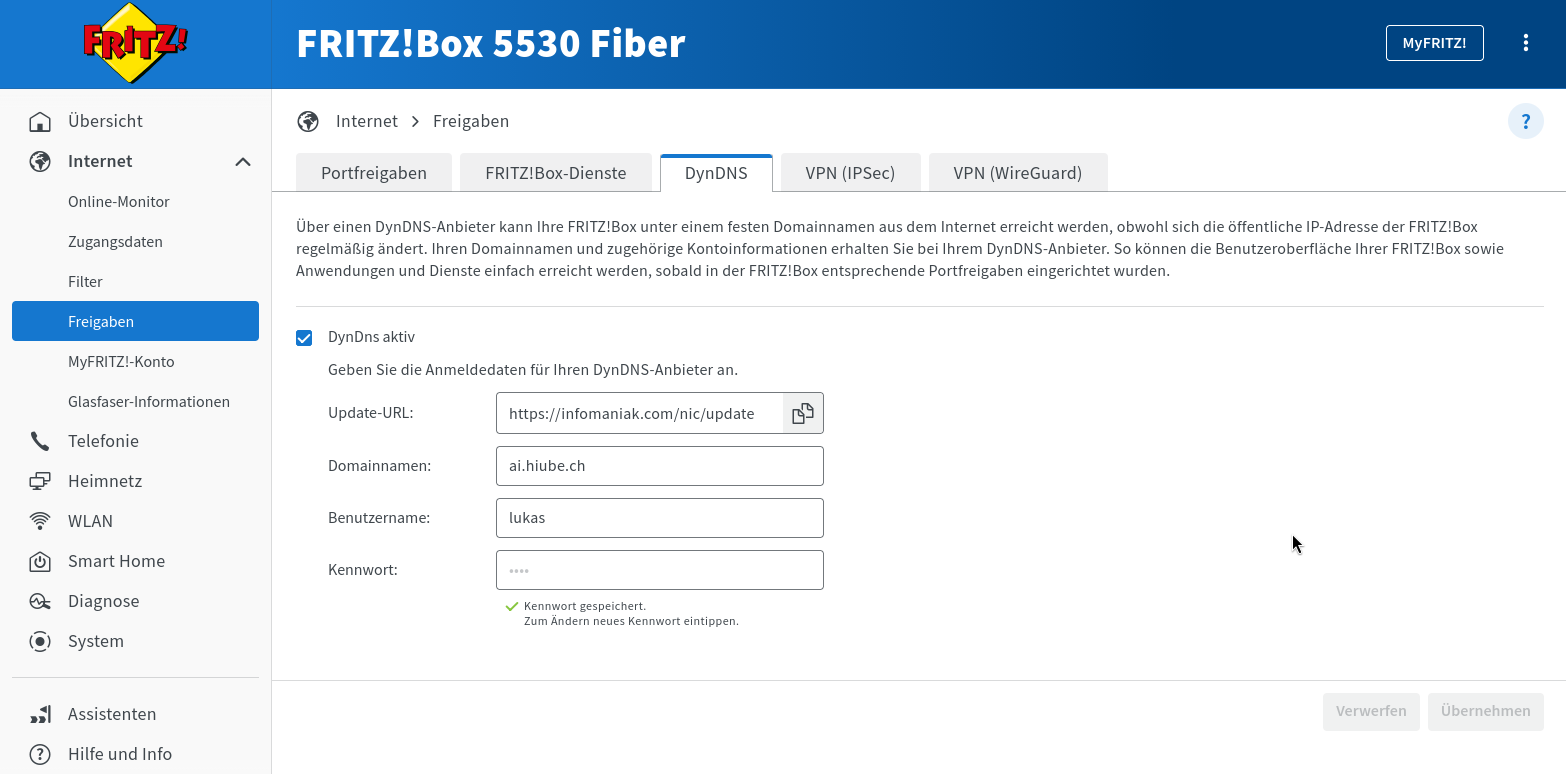
\includegraphics[width=0.8\linewidth]{../assets/screenshots/selfhosted_llm/fritzbox_dyndns_setup}
    \caption{FRITZ!Box DynDNS Setup}
    \label{fig:fritzbox_dyndns_setup}
\end{figure}

\begin{figure}[H]
    \centering
    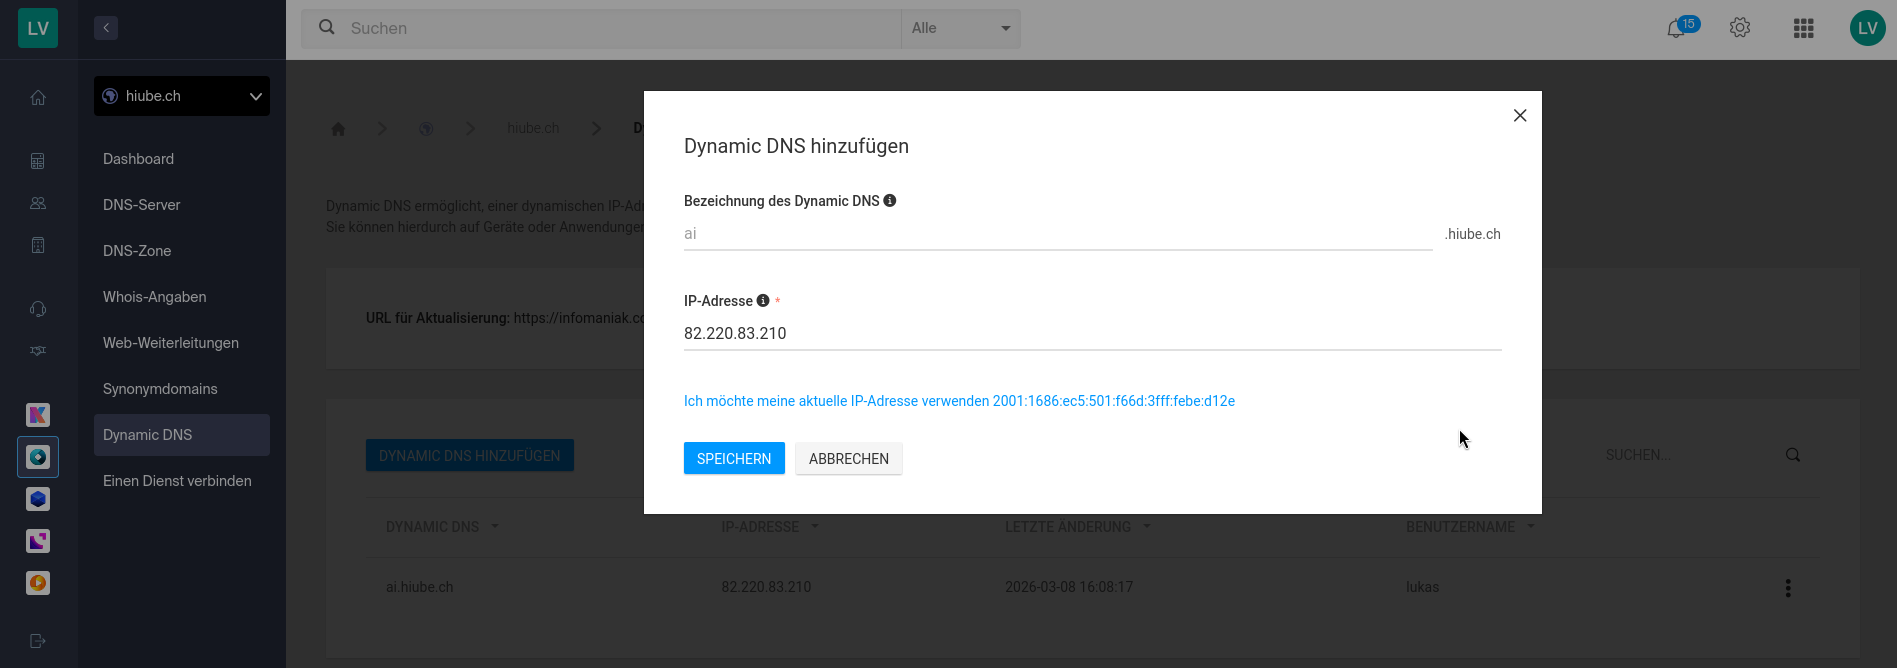
\includegraphics[width=1.0\linewidth]{../assets/screenshots/selfhosted_llm/infomaniak_dyndns_setup}
    \caption{Infomaniak DynDNS Setup}
    \label{fig:infomaniak_dyndns_setup}
\end{figure}

Now that the domain name \enquote{ai.hiube.ch} points to the router in the home network, we need to redirect the HTTP(S) traffic to the \glsxtrshort{LLM} server.
This can be achieved with port forwarding rules on the \gls{FRITZ!Box}, as shown in the screenshot~\ref{fig:fritzbox_port_forwarding}.

\begin{figure}[H]
    \centering
    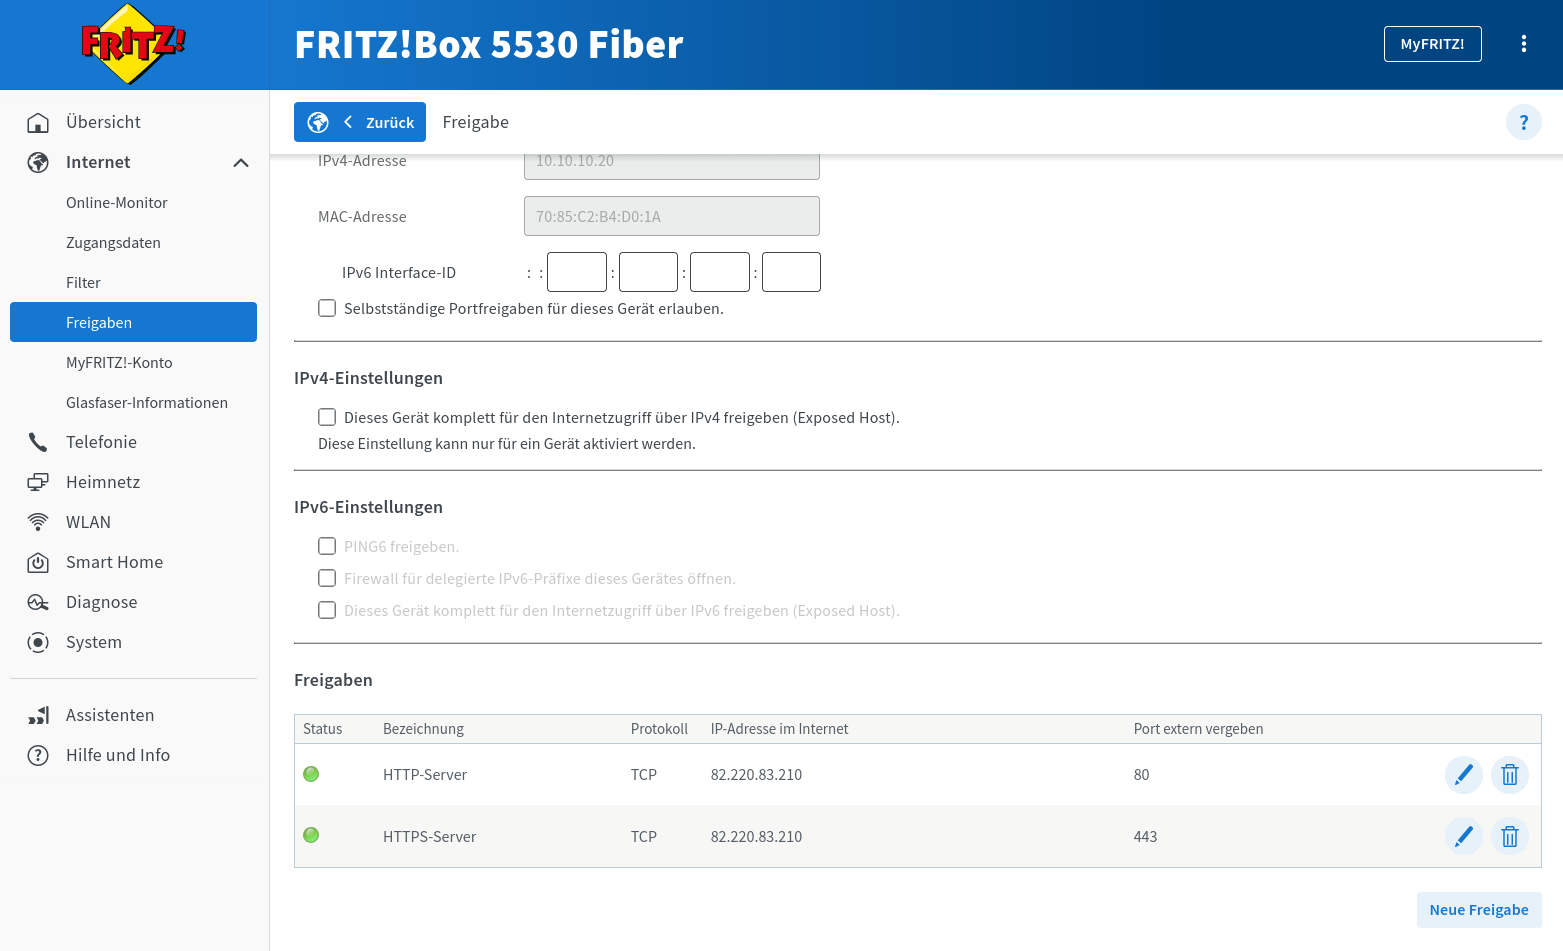
\includegraphics[width=0.8\linewidth]{../assets/screenshots/selfhosted_llm/fritzbox_port_forwarding}
    \caption{FRITZ!Box Port Forwarding}
    \label{fig:fritzbox_port_forwarding}
\end{figure}

The Open WebUI and Ollama \gls{API} should already be reachable via \enquote{ai.hiube.ch}, but we will receive a security warning because there is no valid SSL certificate.
The easiest way to generate the certificate, is to trigger certbot by restarting the \enquote{swag} service as shown in the listing below~\ref{lst:restart-swag-container}.\\

\begin{listing}[H]
    \begin{minted}{bash}
# Login as user ai and restart the swag service
podman-compose restart swag
    \end{minted}
    \caption{Restart SWAG Container}
    \label{lst:restart-swag-container}
\end{listing}

\section{Evaluation}\label{sec:evaluation}

For quickly evaluate models and assess their capabilities we can now use the Open WebUI served under \enquote{ai.hiube.ch}.
The screenshot~\ref{fig:open_webui_evaluation} shows a quick test with \enquote{qwen2.5-coder:7B}.

\begin{figure}[H]
    \centering
    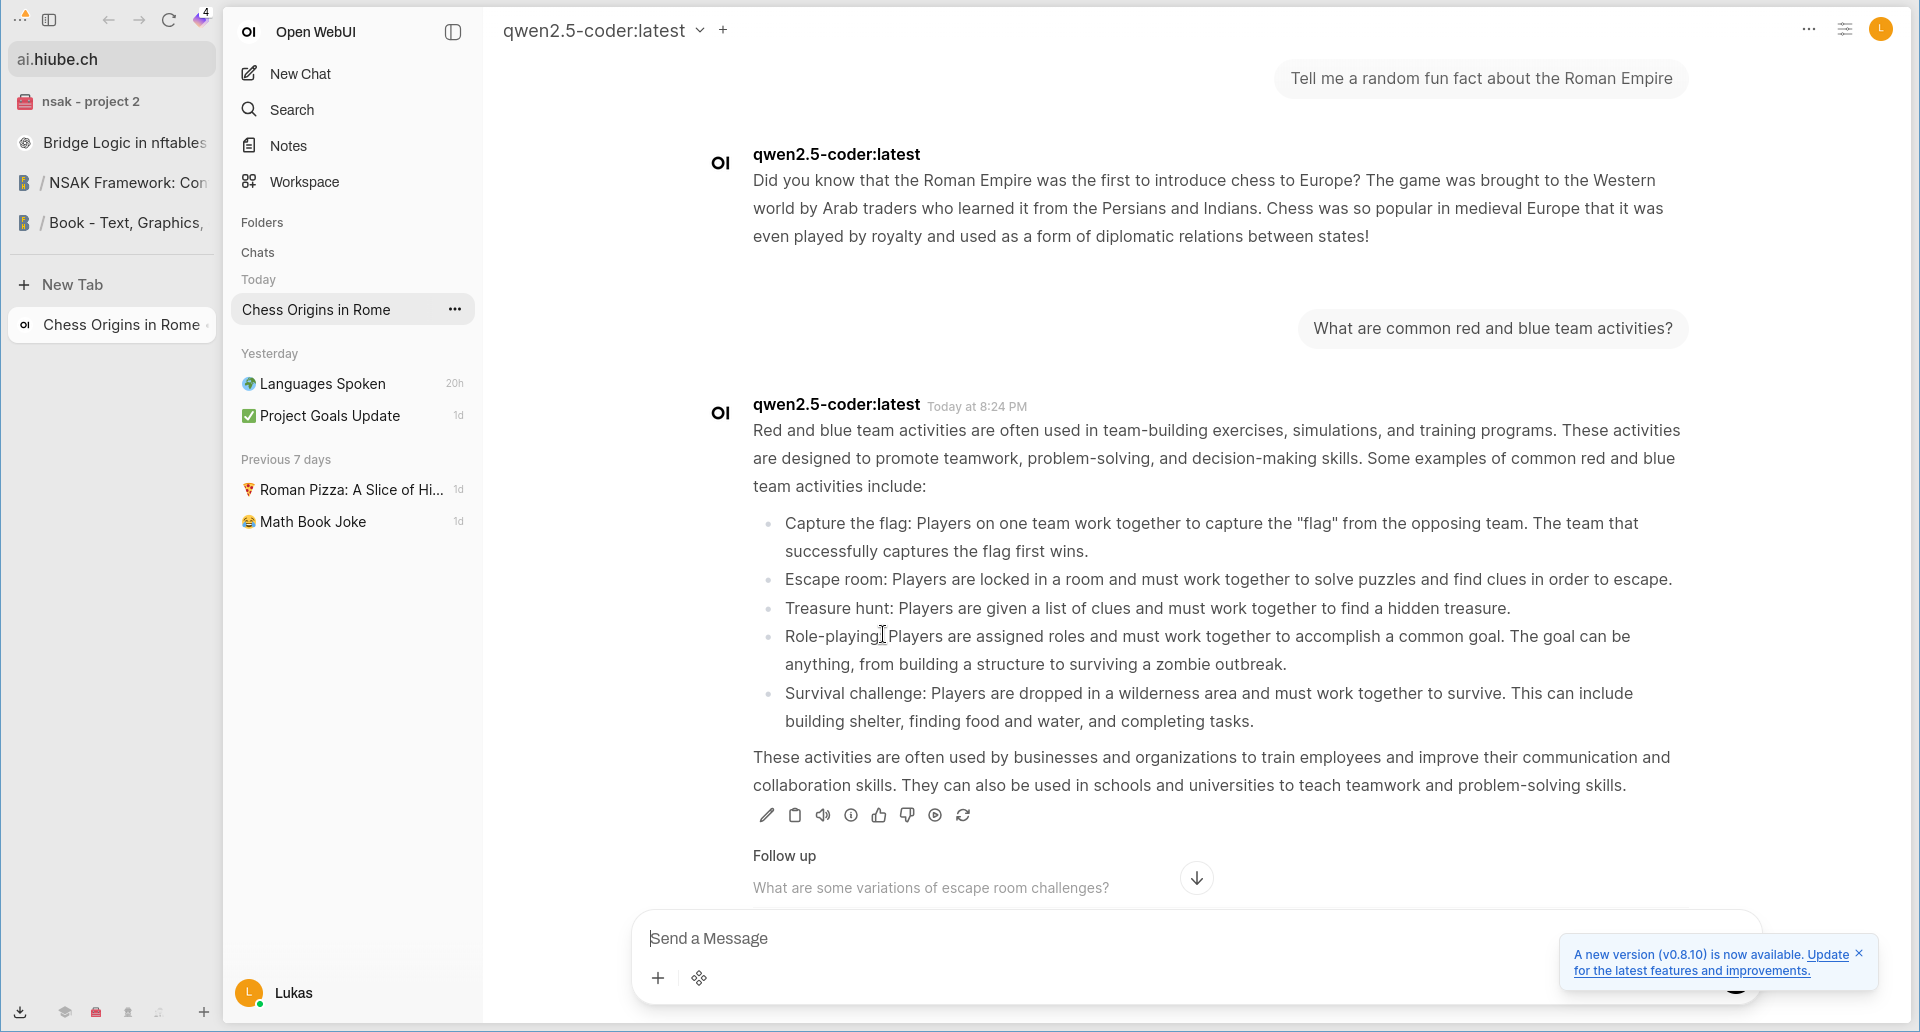
\includegraphics[width=0.8\linewidth]{../assets/screenshots/selfhosted_llm/open_webui_evaluation}
    \caption{OpenWeb UI Evaluation}
    \label{fig:open_webui_evaluation}
\end{figure}

Later on we can use the Ollama \gls{API} served under \mintinline{bash}{/llm/} as a backend for \glsxtrshort{AI} agents.

\newpage
\subsection{Self-Hosted Base Setup}\label{subsec:self-hosted-base-setup}

\begin{listing}[H]
    \inputminted{bash}{listings/self_hosted_nginx/instructions.bash}
    \caption{Self-Hosted Base Setup}
    \label{lst:self-hosted-base-setup-instructions}
\end{listing}

\newpage
\begin{listing}[H]
    \inputminted{bash}{listings/self_hosted_nginx/instructions.bash}
    \caption{Nginx \& Let's Encrypt Instructions}
    \label{lst:nginx-and-lets-encrypt-instructions}
\end{listing}

\newpage
\subsection{Nginx \& Let's Encrypt - Reverse Proxy with SSL Termination}\label{subsec:nginx-and-let's-encrypt-reverse-proxy-with-ssl-termination}

\begin{listing}[H]
    \inputminted{yaml}{listings/self_hosted_nginx/compose.yaml}
    \caption{Nginx \& Let's Encrypt Compose File}
    \label{lst:nginx-and-lets-encrypt-compose-yml}
\end{listing}

\newpage
\subsection{Ollama - LLM Server}\label{subsec:ollama-llm-server}

\begin{listing}[H]
    \inputminted{bash}{listings/self_hosted_ollama/instructions.bash}
    \caption{Ollama Instructions}
    \label{lst:ollama-instructions}
\end{listing}

\newpage
\begin{listing}[H]
    \inputminted{bash}{listings/self_hosted_ollama/nginx.conf}
    \caption{Ollama Nginx Configuration}
    \label{lst:ollama-nginx-conf}
\end{listing}

\newpage
\begin{listing}[H]
    \inputminted{bash}{listings/self_hosted_ollama/enable_ollama_debug_logs.md}
    \caption{Ollama Enable Debug Log}
    \label{lst:ollama-enable-debug-log}
\end{listing}

\newpage
\subsection{Open WebUI - Web Chat for LLM Servers}\label{subsec:open-webui---web-chat-for-llm-servers}

\begin{listing}[H]
    \inputminted{bash}{listings/self_hosted_openwebui/instructions.bash}
    \caption{Open WebUI Instructions}
    \label{lst:open-webui-instructions}
\end{listing}

\newpage
\begin{listing}[H]
    \inputminted{yaml}{listings/self_hosted_openwebui/compose.yaml}
    \caption{Open WebUI Compose File}
    \label{lst:open-webui-compose-yml}
\end{listing}

\newpage
\begin{listing}[H]
    \inputminted{yaml}{listings/self_hosted_openwebui/nginx.conf}
    \caption{Open WebUI Nginx Configuration}
    \label{lst:open-webui-nginx-conf}
\end{listing}

\newpage
\subsection{Drawio MCP - Diagram Tool}\label{subsec:drawio-mcp-diagram-tool}

\begin{listing}[H]
    \inputminted{bash}{listings/self_hosted_drawio/instructions.bash}
    \caption{Drawio Instructions}
    \label{lst:drawio-instructions}
\end{listing}

\begin{listing}[H]
    \inputminted{yaml}{listings/self_hosted_drawio/compose.yaml}
    \caption{Drawio Compose File}
    \label{lst:drawio-compose-yml}
\end{listing}

\begin{listing}[H]
    \inputminted{yaml}{listings/self_hosted_drawio/nginx.conf}
    \caption{Drawio Nginx Configuration}
    \label{lst:drawio-nginx-conf}
\end{listing}

\newpage
\subsection{Grafana / Loki - Logging System}\label{subsec:grafana-loki-logging-system}

\begin{listing}[H]
    \inputminted{bash}{listings/self_hosted_loki/instructions.bash}
    \caption{Grafana / Loki Instructions}
    \label{lst:grafana-loki-instructions}
\end{listing}

\newpage
\begin{listing}[H]
    \inputminted[lastline=59]{yaml}{listings/self_hosted_loki/compose.yaml}
    \caption{Grafana / Loki Compose File: 1/3}
    \label{lst:grafana-loki-compose-yml-1}
\end{listing}

\newpage
\begin{listing}[H]
    \inputminted[firstline=61, lastline=125]{yaml}{listings/self_hosted_loki/compose.yaml}
    \caption{Grafana / Loki Compose File: 2/3}
    \label{lst:grafana-loki-compose-yml-2}
\end{listing}

\newpage
\begin{listing}[H]
    \inputminted[firstline=127]{yaml}{listings/self_hosted_loki/compose.yaml}
    \caption{Grafana / Loki Compose File: 3/3}
    \label{lst:grafana-loki-compose-yml-3}
\end{listing}

\newpage
\begin{listing}[H]
    \inputminted{yaml}{listings/self_hosted_loki/nginx.conf}
    \caption{Grafana / Loki Nginx Configuration}
    \label{lst:grafana-loki-nginx-conf}
\end{listing}

\newpage
\begin{listing}[H]
    \inputminted{yaml}{listings/self_hosted_loki/loki-config.yaml}
    \caption{Grafana / Loki Configuration}
    \label{lst:grafana-loki-config}
\end{listing}

\newpage
\begin{listing}[H]
    \inputminted{yaml}{listings/self_hosted_loki/loki-config.yaml}
    \caption{Grafana / Loki Alloy Configuration}
    \label{lst:grafana-loki-alloy-config}
\end{listing}

